
%% bare_conf.tex
%% V1.3
%% 2007/01/11
%% by Michael Shell
%% See:
%% http://www.michaelshell.org/
%% for current contact information.
%%
%% This is a skeleton file demonstrating the use of IEEEtran.cls
%% (requires IEEEtran.cls version 1.7 or later) with an IEEE conference paper.
%%
%% Support sites:
%% http://www.michaelshell.org/tex/ieeetran/
%% http://www.ctan.org/tex-archive/macros/latex/contrib/IEEEtran/
%% and
%% http://www.ieee.org/

%%*************************************************************************
%% Legal Notice:
%% This code is offered as-is without any warranty either expressed or
%% implied; without even the implied warranty of MERCHANTABILITY or
%% FITNESS FOR A PARTICULAR PURPOSE! 
%% User assumes all risk.
%% In no event shall IEEE or any contributor to this code be liable for
%% any damages or losses, including, but not limited to, incidental,
%% consequential, or any other damages, resulting from the use or misuse
%% of any information contained here.
%%
%% All comments are the opinions of their respective authors and are not
%% necessarily endorsed by the IEEE.
%%
%% This work is distributed under the LaTeX Project Public License (LPPL)
%% ( http://www.latex-project.org/ ) version 1.3, and may be freely used,
%% distributed and modified. A copy of the LPPL, version 1.3, is included
%% in the base LaTeX documentation of all distributions of LaTeX released
%% 2003/12/01 or later.
%% Retain all contribution notices and credits.
%% ** Modified files should be clearly indicated as such, including  **
%% ** renaming them and changing author support contact information. **
%%
%% File list of work: IEEEtran.cls, IEEEtran_HOWTO.pdf, bare_adv.tex,
%%                    bare_conf.tex, bare_jrnl.tex, bare_jrnl_compsoc.tex
%%*************************************************************************

% *** Authors should verify (and, if needed, correct) their LaTeX system  ***
% *** with the testflow diagnostic prior to trusting their LaTeX platform ***
% *** with production work. IEEE's font choices can trigger bugs that do  ***
% *** not appear when using other class files.                            ***
% The testflow support page is at:
% http://www.michaelshell.org/tex/testflow/




% Note that the a4paper option is mainly intended so that authors in
% countries using A4 can easily print to A4 and see how their papers will
% look in print - the typesetting of the document will not typically be
% affected with changes in paper size (but the bottom and side margins will).
% Use the testflow package mentioned above to verify correct handling of
% both paper sizes by the user's LaTeX system.
%
% Also note that the "draftcls" or "draftclsnofoot", not "draft", option
% should be used if it is desired that the figures are to be displayed in
% draft mode.
%
\documentclass[10pt, conference, compsocconf]{IEEEtran}
% Add the compsocconf option for Computer Society conferences.
%
% If IEEEtran.cls has not been installed into the LaTeX system files,
% manually specify the path to it like:
% \documentclass[conference]{../sty/IEEEtran}
% Some very useful LaTeX packages include:
% (uncomment the ones you want to load)


% *** MISC UTILITY PACKAGES ***
%
%\usepackage{ifpdf}
% Heiko Oberdiek's ifpdf.sty is very useful if you need conditional
% compilation based on whether the output is pdf or dvi.
% usage:
% \ifpdf
%   % pdf code
% \else
%   % dvi code
% \fi
% The latest version of ifpdf.sty can be obtained from:
% http://www.ctan.org/tex-archive/macros/latex/contrib/oberdiek/
% Also, note that IEEEtran.cls V1.7 and later provides a builtin
% \ifCLASSINFOpdf conditional that works the same way.
% When switching from latex to pdflatex and vice-versa, the compiler may
% have to be run twice to clear warning/error messages.






% *** CITATION PACKAGES ***
%
\usepackage{cite}
% cite.sty was written by Donald Arseneau
% V1.6 and later of IEEEtran pre-defines the format of the cite.sty package
% \cite{} output to follow that of IEEE. Loading the cite package will
% result in citation numbers being automatically sorted and properly
% "compressed/ranged". e.g., [1], [9], [2], [7], [5], [6] without using
% cite.sty will become [1], [2], [5]--[7], [9] using cite.sty. cite.sty's
% \cite will automatically add leading space, if needed. Use cite.sty's
% noadjust option (cite.sty V3.8 and later) if you want to turn this off.
% cite.sty is already installed on most LaTeX systems. Be sure and use
% version 4.0 (2003-05-27) and later if using hyperref.sty. cite.sty does
% not currently provide for hyperlinked citations.
% The latest version can be obtained at:
% http://www.ctan.org/tex-archive/macros/latex/contrib/cite/
% The documentation is contained in the cite.sty file itself.






% *** GRAPHICS RELATED PACKAGES ***
%
\ifCLASSINFOpdf
   \usepackage[pdftex]{graphicx}
  % declare the path(s) where your graphic files are
   \graphicspath{{../pdf/}{../jpeg/}}
  % and their extensions so you won't have to specify these with
  % every instance of \includegraphics
   \DeclareGraphicsExtensions{.pdf,.jpeg,.png}
   \DeclareGraphicsRule{*}{mps}{*}{}
\else
  % or other class option (dvipsone, dvipdf, if not using dvips). graphicx
  % will default to the driver specified in the system graphics.cfg if no
  % driver is specified.
   \usepackage[dvips]{graphicx}
  % declare the path(s) where your graphic files are
   \graphicspath{{./}}
  % and their extensions so you won't have to specify these with
  % every instance of \includegraphics
   \DeclareGraphicsExtensions{.png, .pdf, .eps}
\fi


% graphicx was written by David Carlisle and Sebastian Rahtz. It is
% required if you want graphics, photos, etc. graphicx.sty is already
% installed on most LaTeX systems. The latest version and documentation can
% be obtained at: 
% http://www.ctan.org/tex-archive/macros/latex/required/graphics/
% Another good source of documentation is "Using Imported Graphics in
% LaTeX2e" by Keith Reckdahl which can be found as epslatex.ps or
% epslatex.pdf at: http://www.ctan.org/tex-archive/info/
%
% latex, and pdflatex in dvi mode, support graphics in encapsulated
% postscript (.eps) format. pdflatex in pdf mode supports graphics
% in .pdf, .jpeg, .png and .mps (metapost) formats. Users should ensure
% that all non-photo figures use a vector format (.eps, .pdf, .mps) and
% not a bitmapped formats (.jpeg, .png). IEEE frowns on bitmapped formats
% which can result in "jaggedy"/blurry rendering of lines and letters as
% well as large increases in file sizes.
%
% You can find documentation about the pdfTeX application at:
% http://www.tug.org/applications/pdftex





% *** MATH PACKAGES ***
%
%\usepackage[cmex10]{amsmath}
% A popular package from the American Mathematical Society that provides
% many useful and powerful commands for dealing with mathematics. If using
% it, be sure to load this package with the cmex10 option to ensure that
% only type 1 fonts will utilized at all point sizes. Without this option,
% it is possible that some math symbols, particularly those within
% footnotes, will be rendered in bitmap form which will result in a
% document that can not be IEEE Xplore compliant!
%
% Also, note that the amsmath package sets \interdisplaylinepenalty to 10000
% thus preventing page breaks from occurring within multiline equations. Use:
%\interdisplaylinepenalty=2500
% after loading amsmath to restore such page breaks as IEEEtran.cls normally
% does. amsmath.sty is already installed on most LaTeX systems. The latest
% version and documentation can be obtained at:
% http://www.ctan.org/tex-archive/macros/latex/required/amslatex/math/





% *** SPECIALIZED LIST PACKAGES ***
%
%\usepackage{algorithmic}
% algorithmic.sty was written by Peter Williams and Rogerio Brito.
% This package provides an algorithmic environment fo describing algorithms.
% You can use the algorithmic environment in-text or within a figure
% environment to provide for a floating algorithm. Do NOT use the algorithm
% floating environment provided by algorithm.sty (by the same authors) or
% algorithm2e.sty (by Christophe Fiorio) as IEEE does not use dedicated
% algorithm float types and packages that provide these will not provide
% correct IEEE style captions. The latest version and documentation of
% algorithmic.sty can be obtained at:
% http://www.ctan.org/tex-archive/macros/latex/contrib/algorithms/
% There is also a support site at:
% http://algorithms.berlios.de/index.html
% Also of interest may be the (relatively newer and more customizable)
% algorithmicx.sty package by Szasz Janos:
% http://www.ctan.org/tex-archive/macros/latex/contrib/algorithmicx/




% *** ALIGNMENT PACKAGES ***
%
%\usepackage{array}
% Frank Mittelbach's and David Carlisle's array.sty patches and improves
% the standard LaTeX2e array and tabular environments to provide better
% appearance and additional user controls. As the default LaTeX2e table
% generation code is lacking to the point of almost being broken with
% respect to the quality of the end results, all users are strongly
% advised to use an enhanced (at the very least that provided by array.sty)
% set of table tools. array.sty is already installed on most systems. The
% latest version and documentation can be obtained at:
% http://www.ctan.org/tex-archive/macros/latex/required/tools/


%\usepackage{mdwmath}
%\usepackage{mdwtab}
% Also highly recommended is Mark Wooding's extremely powerful MDW tools,
% especially mdwmath.sty and mdwtab.sty which are used to format equations
% and tables, respectively. The MDWtools set is already installed on most
% LaTeX systems. The lastest version and documentation is available at:
% http://www.ctan.org/tex-archive/macros/latex/contrib/mdwtools/


% IEEEtran contains the IEEEeqnarray family of commands that can be used to
% generate multiline equations as well as matrices, tables, etc., of high
% quality.


%\usepackage{eqparbox}
% Also of notable interest is Scott Pakin's eqparbox package for creating
% (automatically sized) equal width boxes - aka "natural width parboxes".
% Available at:
% http://www.ctan.org/tex-archive/macros/latex/contrib/eqparbox/





% *** SUBFIGURE PACKAGES ***
%\usepackage[tight,footnotesize]{subfigure}
% subfigure.sty was written by Steven Douglas Cochran. This package makes it
% easy to put subfigures in your figures. e.g., "Figure 1a and 1b". For IEEE
% work, it is a good idea to load it with the tight package option to reduce
% the amount of white space around the subfigures. subfigure.sty is already
% installed on most LaTeX systems. The latest version and documentation can
% be obtained at:
% http://www.ctan.org/tex-archive/obsolete/macros/latex/contrib/subfigure/
% subfigure.sty has been superceeded by subfig.sty.



%\usepackage[caption=false]{caption}
%\usepackage[font=footnotesize]{subfig}
% subfig.sty, also written by Steven Douglas Cochran, is the modern
% replacement for subfigure.sty. However, subfig.sty requires and
% automatically loads Axel Sommerfeldt's caption.sty which will override
% IEEEtran.cls handling of captions and this will result in nonIEEE style
% figure/table captions. To prevent this problem, be sure and preload
% caption.sty with its "caption=false" package option. This is will preserve
% IEEEtran.cls handing of captions. Version 1.3 (2005/06/28) and later 
% (recommended due to many improvements over 1.2) of subfig.sty supports
% the caption=false option directly:
%\usepackage[caption=false,font=footnotesize]{subfig}
%
% The latest version and documentation can be obtained at:
% http://www.ctan.org/tex-archive/macros/latex/contrib/subfig/
% The latest version and documentation of caption.sty can be obtained at:
% http://www.ctan.org/tex-archive/macros/latex/contrib/caption/




% *** FLOAT PACKAGES ***
%
%\usepackage{fixltx2e}
% fixltx2e, the successor to the earlier fix2col.sty, was written by
% Frank Mittelbach and David Carlisle. This package corrects a few problems
% in the LaTeX2e kernel, the most notable of which is that in current
% LaTeX2e releases, the ordering of single and double column floats is not
% guaranteed to be preserved. Thus, an unpatched LaTeX2e can allow a
% single column figure to be placed prior to an earlier double column
% figure. The latest version and documentation can be found at:
% http://www.ctan.org/tex-archive/macros/latex/base/



%\usepackage{stfloats}
% stfloats.sty was written by Sigitas Tolusis. This package gives LaTeX2e
% the ability to do double column floats at the bottom of the page as well
% as the top. (e.g., "\begin{figure*}[!b]" is not normally possible in
% LaTeX2e). It also provides a command:
%\fnbelowfloat
% to enable the placement of footnotes below bottom floats (the standard
% LaTeX2e kernel puts them above bottom floats). This is an invasive package
% which rewrites many portions of the LaTeX2e float routines. It may not work
% with other packages that modify the LaTeX2e float routines. The latest
% version and documentation can be obtained at:
% http://www.ctan.org/tex-archive/macros/latex/contrib/sttools/
% Documentation is contained in the stfloats.sty comments as well as in the
% presfull.pdf file. Do not use the stfloats baselinefloat ability as IEEE
% does not allow \baselineskip to stretch. Authors submitting work to the
% IEEE should note that IEEE rarely uses double column equations and
% that authors should try to avoid such use. Do not be tempted to use the
% cuted.sty or midfloat.sty packages (also by Sigitas Tolusis) as IEEE does
% not format its papers in such ways.





% *** PDF, URL AND HYPERLINK PACKAGES ***
%
%\usepackage{url}
% url.sty was written by Donald Arseneau. It provides better support for
% handling and breaking URLs. url.sty is already installed on most LaTeX
% systems. The latest version can be obtained at:
% http://www.ctan.org/tex-archive/macros/latex/contrib/misc/
% Read the url.sty source comments for usage information. Basically,
% \url{my_url_here}.





% *** Do not adjust lengths that control margins, column widths, etc. ***
% *** Do not use packages that alter fonts (such as pslatex).         ***
% There should be no need to do such things with IEEEtran.cls V1.6 and later.
% (Unless specifically asked to do so by the journal or conference you plan
% to submit to, of course. )


% correct bad hyphenation here
\hyphenation{op-tical net-works semi-conduc-tor}


\begin{document}
%
% paper title
% can use linebreaks \\ within to get better formatting as desired
\title{A Template Metaprogramming Approach to Support Parallel Programs for Multicores}
% author names and affiliations
% use a multiple column layout for up to two different
% affiliations

%\author{\IEEEauthorblockN{Authors Name/s per 1st Affiliation (Author)}
%\IEEEauthorblockA{line 1 (of Affiliation): dept. name of organization\\
%line 2: name of organization, acronyms acceptable\\
%line 3: City, Country\\
%line 4: Email: name@xyz.com}
%\and
%\IEEEauthorblockN{Authors Name/s per 2nd Affiliation (Author)}
%\IEEEauthorblockA{line 1 (of Affiliation): dept. name of organization\\
%line 2: name of organization, acronyms acceptable\\
%line 3: City, Country\\
%line 4: Email: name@xyz.com}
%}

% conference papers do not typically use \thanks and this command
% is locked out in conference mode. If really needed, such as for
% the acknowledgment of grants, issue a \IEEEoverridecommandlockouts
% after \documentclass

% for over three affiliations, or if they all won't fit within the width
% of the page, use this alternative format:
% 
\author{
\IEEEauthorblockN{Xin Liu, Daqiang Zhang, Jingyu Zhou, Minyi Guo, Yao Shen}
\IEEEauthorblockA{Department of Computer Science\\
Shanghai Jiao Tong University\\
No. 800, Dongchuan Road, Shanghai, P.R.China\\
\{navyliu, zhangdq\}@sjtu.edu.cn, \{guo-my, zhou-jy, shen\_yao\}@cs.sjtu.edu.cn}
}

% use for special paper notices
%\IEEEspecialpapernotice{(Invited Paper)}

% make the title area
\maketitle


\begin{abstract}
In advent of multicore era, plain C/C++ programming language can not
fully reflect computer architectures any more. Source-to-source
transformation helps tailor programs close to contemporary
hardwares. We propose a template-based approach to perform 
transformation for programs with rich static information.
The template metaprogramming techniques we present can conduct
parallelization and memory hierarchical optimization for specific multicores. They enable
programmers to utilize new architectural
features and parallel patterns by extending template library. 
In this paper, we implement a prototype template library -- libvina
to demonstrate the idea. Finally, We evaluate our template library on
commodity x86 and GPU platforms by a variety of typical applications
in multimedia and scientific fields. In experiments, we show that our
approach is flexible to support multiple parallel models and capable
of transforming sequential code to parallel equivalence  according to
specific multicore architectures. Moreover, the cost of programmability using our
approach to adapt more than one multicore platform is manageable.
% In addition, the experimental results reveal that our approach incurs little run-time overhead because it takes effects in compile-time.
\end{abstract}

\begin{IEEEkeywords}
static analysis; source-to-souce transformation; parallelization; multicore; metaprogramming
\end{IEEEkeywords}


% For peer review papers, you can put extra information on the cover
% page as needed:
% \ifCLASSOPTIONpeerreview
% \begin{center} \bfseries EDICS Category: 3-BBND \end{center}
% \fi
%
% For peerreview papers, this IEEEtran command inserts a page break and
% creates the second title. It will be ignored for other modes.
\IEEEpeerreviewmaketitle

\section{Introduction}
Multicores rely on parallelism and memory
hierarchy to improve performance. Both duplicated processors and
elaborated storage-on-chip require programmers to restructure their
source code and keep tuning binaries for a specific target. Therefore,
non-trivial knowledge of underlying machine's architectures is
necessary to write high-performance applications. More worse, various
implementations of multicores bring many architectural
features to programmers, which in fact further enlarge the gap between software
programmers and hardware vendors.

Traditionally, algorithm experts usually focus on their specific domains and have
limited insights on diverging computer systems. Writing algorithms in
sequence, they expect hardwares
and compilers to guarantee decent performance for their
programs. The expectation was roughly held until explicit parallel system was
introduced to computer community. Since the frequency of microprocessor
increases slowly, it has been difficult to obtain free
performance improvement from hardware's refinement. Workloads
of application developers surge for parallel computer
systems. In essence, it is because plain C/C++ can not fully reflect contemporary
parallel architectures. It is desirable to develop
methods to adapt to diverging multicore architectures.

Although extensive researches on non-traditional
programming models obtain fruitful achievements, mainstream software development still
stay at imperative programming languages and multi-threading.
We think the primary reason is software cost. Considering the time span
which a large computer system serves, hardwares are cheap and become
cheaper with time elapsing, while software and well-trained personnel are
expensive. Because numerous legacy software systems were designed and
developed in conventional programming model, vendors usually prefer to
maintain and update them rather than
rebuilding from scratch. Nevertheless, exploiting horsepower of
multicore processors for legacy and new systems is a moderate issue.

%Designing new parallel programming language
%is approachable. Many functional languages with inherent supports for
%concurrency have emerged in the horizon. 

%Researchers have admitted that it is
%tremendously challenging for optimizing sequential code only relying
%on compilers, so the answer to bridge programmer to multicore hardware
%moves to that language and library express parallelism and
%concurrency richer than ever.

%One side, software developers insist on classic programming diagrams
%and are reluctant to rewrite existing sources. On the other side,
%exploiting horsepower of multicore processors for existing and new
%systems is a moderate issue. Therefore, it is desirable to extend
%traditional programming languages for the trade-off.

%Many programming languages extending C/C++ had been proposed for
%multicore. However,  existing ad-hoc approaches are either only
%capable of one parallel pattern or on one hardware
%platform. OpenMP supports CUDA~\cite{cudaref} and Brook~\cite{brookgpu} works on vender-dependent GPU architectures for streaming
%computation. ~\cite{saha09} is for heterogenous x86 platform.

Source-to-source transformation can help tailor specific
architectures. In particular, some transformations can extend
traditional programming language to support multicore
architectures. OpenMP~\cite{openmp} and Sequoia~\cite{sequoia, sequoia-compiler}
are typical examples. One distinct attribute comparing with other
fancy languages is that they
support progressive parallelization from original source code, which
can guarantee to keep software investment. OpenMP transform program regions into fork-join threads based on
pragma directives. Sequoia attempts to map computation-intensive functions
on a machine tree describing in configuration file. In those
extended languages,  a set of language
constructs are provided to support specific parallel patterns, so they
need dedicated compilers. Instead of modifying compiler and introducing new language constructs, we exploit
the capability of C++ template mechanism to achieve source-to-source
transformation. All transformations are programmed in C++ metaprogramming
\cite{tempmetaprog} and are conducted by a group of template classes
when that are instantiated. The primary limitation is that only static
information are available at compile time. Therefore, it only works for programs which own rich static information. Fortunately, applications with this characteristic are pervasive in multimedia, digital processing, and scientific computation.

Because template takes effect at compile time, it is possible to avoid
deploying run-time for transformation, which means that it can incur minimal
runtime cost. Besides, our template-based approach imposes fewer restricts comparing with other static approaches:

\begin{itemize}
\item Flexibility: We proposed a way to perform source-to-source transformation by
metaprogramming. Because it can manipulate source code in metaprograms,  our approach does not bind any parallel models. It is easy to
change transform to fork-join, or perform computation
as pipeline. In addition, our approach can deploy any thread
implementations to support parallelism and concurrency. We experiment
pthread, low-level threads provided by OS and device driver. As far as we know, no parallel programming language
declares such flexibility. Theoretically, metaprogramming is
as expressive as any general-purposed programming languages, so we
think it is a promising approach to explore more parallel patterns
beyond this paper.

\item Extendability:  It is extensible to develop new template class to
  utilize new architectural features  and parallel patterns. Template
  metaprogramming is intimate for C++ programmers. It is easy to
  extend new execution models and parallel patterns. Other approaches
  have to ratify languages and then modify compiler to complete
  features. The progress is usually a year-old compaign and can not
  determined by software developers alone.

\item Portability: Template is part of ISO C++~\cite{c++03, c++0x}. Template-based approach is applicable for every
  platforms with standard C++ compiler. Template metaprogramming is
  widely used in other applications in C++ community and full-blown
  metaprogramming libraries like
  MPL~\cite{mpl} is portable. Through good encapsulation of
  platform details, most of code in our template approach can be reused.
\end{itemize}

%organization structure
The remaining parts of this paper are structured as follows.
 Section 2 shows techniques to perform
transforms by template metaprogramming. Audiences with C++ template
programming experiences or functional programming language concepts
are helpful but not prerequisites. Then Section 3 presents some
typical transformations by our template library. Experiments are in
Section 4 to evaluate performance on both CPU and GPU.
Section 5 summarizes some related works on library-based approach and
language extension to support multicore architectures.  The last section is conclusion and future work.
\section{Template Metaprogramming Approach}
\subsection{Background}
%template general
Originally, C++ template mechanism is invented to supersede C
preprocessor. It is type-safed and could facility generic
programming. People found the potential of template computation by
chance. \cite{tempturing} later proved template itself is Turing
completeness. Beside the job it meant to do, template has been successfully applied to many innovative purposes in modern C++ programming practices \cite{moderncpp}. 

%template sepcialization
A powerful feature of C++'s templates is \emph{template specialization}. This allows alternative implementations to be provided based on certain characteristics of the parameterized type that is being instantiated. Template specialization has two purposes: to allow certain forms of optimization, and to reduce code bloat ~\cite{tcpl}.

%template metaprogramming 
\emph{Metaprogramming} is the writing of computer programs that write or
manipulate other programs(or themselves) as their data. \emph{C++ Template
 metaprogramming} is metaprograming by template techniques in
C++ programming language. It is similar to functional programming
language except it takes effect at compile time. It only relies on
static information to determine control flow and perform
computation. MPL Library \cite{mpl, tempmetaprog} provides language
constructs and STL-like data structures corresponding to conventional
C++ program, which significantly eases
programming in static realm.

% seqpar seqreduce
\subsection{Overview}
\begin{figure}[htp]
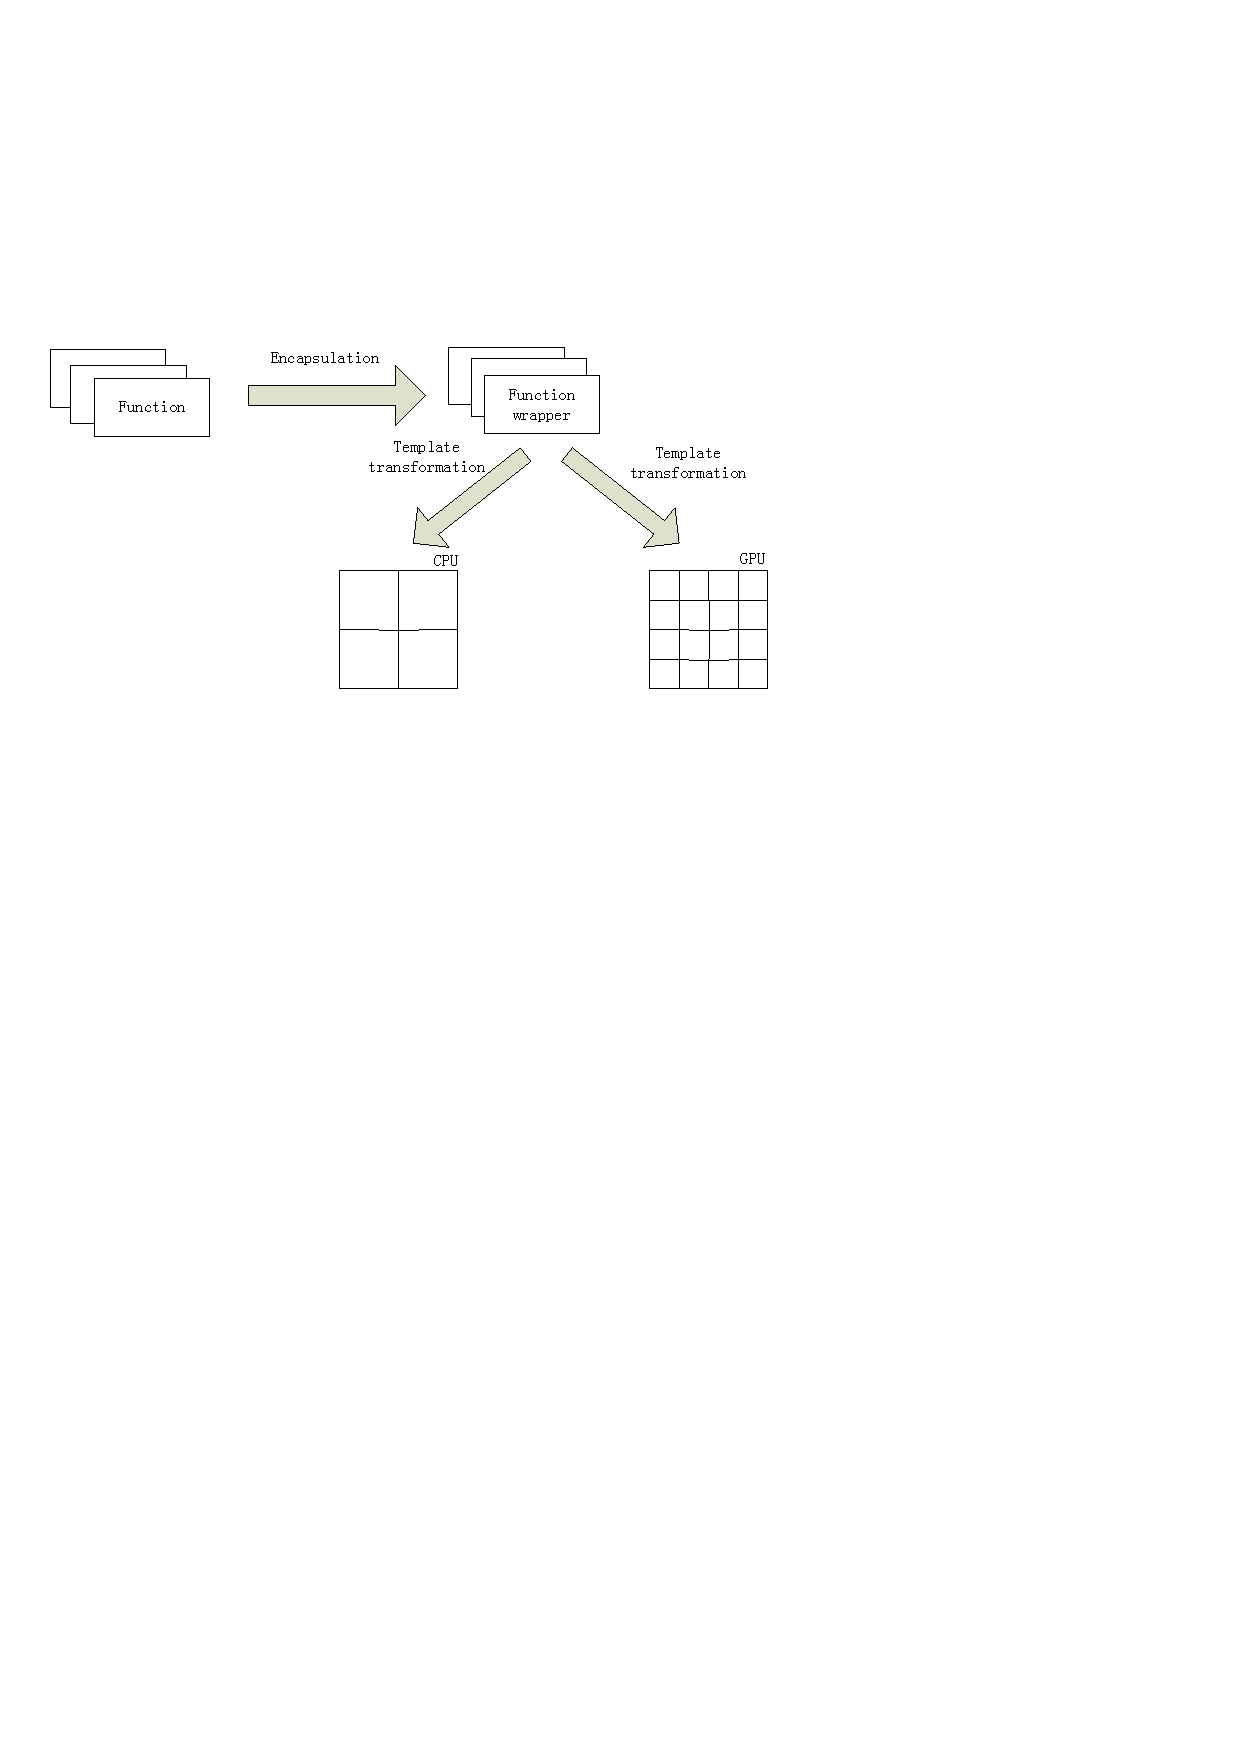
\includegraphics[width=3.3in]{overview}
\caption{template transformation}\label{fig:overview}
\end{figure}
%separation of roles.
Fig.~\ref{fig:overview} is the diagram of source-to-source
transformation using template metaprogramming. In our design philosophy, we separate two roles in software
development. Algorithm programmers are application-specific experts,
who are only concerned about efficient algorithms in conventional
C/C++ form. They provide functions in the form of function wrappers. So
the encapsulation process is achieved by algorithm programmers. On the other side, system
programmer who know underlying computer architectures write C++
template library to take responsibility for transformation. We extend
the concept of template specialization to multicore architectures.
Specializations of a function wrapper for different architectures are
achieved by applying a series of template classes. A regular C++ compiler
can transform source codes according to deployed templates.

%mechnism
One foundation of our approach is to assume C++
compiler front-end as a code generator. It actually practices
source-to-source transformation in the guidance of template
metaprogramming. Function wrappers are parametric with respect to
template arguments instead of function arguments. This enables
C++ compiler manipulate  functions at compile time. 

%introduce libvina for cpu and gpu.
We implemented a prototype template library -- libvina, to perform source-to-source
transformation for both CPU and GPU. On CPU, we define template
classes recursively to generate variants for a function wrapper. On GPU, things became trivial because GPUs map and
manage massive number of threads by hardware. Transformations are
abstracted by metaprograms and are organized as a template
library. Template library such as libvina enables to re-use
the repetitive efforts of system programmers.  Porting
from one platform to another usually  only need to adjust
template arguments or apply another group of template classes. It is not necessary to
dig into algorithms to explore parallelism again. As depicted in
Fig. ~\ref{fig:overview}, we apply different template classes to
transform the same function wrappers for CPU and GPU respectively.


%As mentioned before, template approach is limited in
%compile time, therefore, problems we intend to solve must have rich static
%information. Fortunately,  applications with this characteristic are
%not uncommon in multimedia or digital processing fields, some of them 
%even attract developers to implement them in hardware such as FPGA or DSP. To leverage
%static information, we provides data structures with
%template parameters to carry such information. 

\subsection{Components}
\subsubsection{TF class}
%TF class
Computation-intensive functions are commonly referred to as
\emph{kernel} or \emph{filter}. Mathematically, a function is
single-target binary relation. Kernel functions are usually
self-contained, \textit{i.e.} external data references are limited and
calling graphs are simple. It's possible for a kernel function to
decouple into a cluster of subprocedures. Each subprocedure may be
exactly the same and spread on multicore to execute in
parallel.  Another approach is to divide a kernel into finer stages
and run in pipeline manner to respect data locality and bandwidth. In
libvina, a \emph{transform class (TF class)} is a template class which
transforms a function to a cluster of subprocedures in isomorphism. As
shown in Fig.~\ref{fig:tfcls}, the transformed function on right side
has the same interface while owns a call graph to complete the
original computation by a cluster of subprocedures. Execution of the
call graph can be programmed by in the library to take advantage of
architectural features.

\begin{figure}
\centering
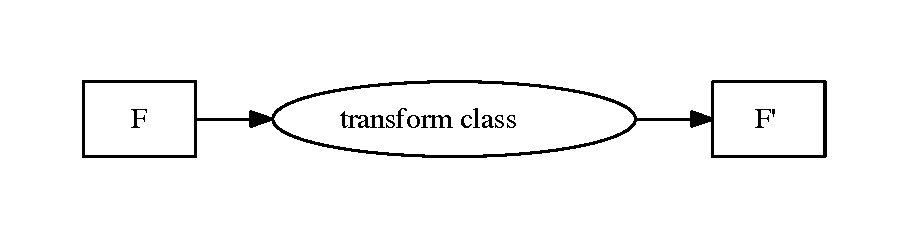
\includegraphics[width=3.1in]{map-class}
\caption{transform class}\label{fig:tfcls}
\end{figure}

\subsubsection{Function wrapper}\label{section:interface}
In programming language, a function which can apply any values of
different types are parametric polymorphism. C++ has already supported
this language feature by template function. Our library needs to
manipulate template functions and instantiate them on demand, which we
call it \emph{late-instantiation} inspired of
\emph{late-binding}. Because the entry address of a template function is not available until instantiation, it is desirable to extend function
polymorphism for different template arguments  at compile-time. Our
approach is to wrap the template function by a template class and pass
it as \emph{template template class}. A wrapper function acts
as interface provided by algorithm developers. Fig.~\ref{lst:wrapper} is a wrapper function of vector addition. 

Beside it enables late-instantiation, the advantage of template class interface
is to provide different entries for different execution environments. \emph{doit\_b} is
used to implement synchronization in Fig.~\ref{fig:mm}.  Another benefit of
this form is that wrapper classes  give compiler a chance to select
appropriate codes based on their types, which is T in our example. This method incurs an extra function call  thought, it is hopefully  eliminated by
compiler's inline optimization.

\begin{figure}[!htp]
\begin{minipage}[tb]{\linewidth}
\makebox[\textwidth]{\hrulefill}
\begin{small}
\begin{verbatim}
/*A function wrapper for vector addition
 */
template<class Result, class Arg0, 
         class Arg1>
struct vecAddWrapper {
 //omitted...
 
 //entry
 static void 
 doit(const Arg0& arg0, const Arg1& arg1, 
     Result& result)
 {
  vecArithImpl<T, DIM_N>::add(arg0, arg1, 
                           result);
 }

 //entry with a barrier to synchronize
 static void 
 doit_b(const Arg0& arg0, const Arg1& arg1, 
     Result& result, mt::barrier& barrier)
 {
   doit(arg0, arg1, result);
   barrier.wait();
 }

 //...
};
\end{verbatim}
\end{small}
\makebox[\textwidth]{\hrulefill}
\end{minipage}
\caption{Function Wrapper}\label{lst:wrapper}
\end{figure}

%predicate and sentinel
\subsubsection{Predicate}
Borrowed from lisp concept, \emph{predicate} represents an indicator
of some conditions. It is a template class with static
fields initialized by constant expressions consisting of template
parameters and constants. These fields are automatically evaluated
when template classes are instantiated. Fig.~\ref{lst:pred} is an example to determine whether the problem size is fitting for last level cache.

\begin{figure}[!htp]
\begin{minipage}[tb]{\linewidth}
\makebox[\textwidth]{\hrulefill}
\begin{small}
\begin{verbatim}
/*determine whether the problem size is 
 *less than last level cache.
 */
template <class T, int SIZE_A
     , int SIZE_B, int SIZE_C>
struct p_lt_cache_ll {
 enum {CACHE_LL_SIZE = 4096*1024};
 const static bool value = 
     ((SIZE_A * SIZE_B 
   + SIZE_A * SIZE_C + SIZE_B * SIZE_C) 
   * sizeof(T) ) <= CACHE_LL_SIZE;
};
\end{verbatim}
\end{small}
\vspace{-1ex}\makebox[\textwidth]{\hrulefill}
\end{minipage}
\caption{Predicate}\label{lst:pred}
\end{figure}

\subsubsection{Sentinel}
\emph{Sentinels} in libvina are non-type template parameters of
\emph{TF class}. When a template class is instantiating, sentinels are
evaluated from a \emph{predicate}.  The \emph{predicate} determines
whether a specific requirement has been satisfied. Sentinel is
responsible for changing generation strategy according to the
result. Using \emph{template specialization}, C++ compiler chooses
different versions of class to instantiate basing on the values or
types of template arguments. The most important application of
\emph{sentinel} is to  terminate recursion. More general flow control
such as branch is available in MPL ~\cite{mpl}.

\subsection{Supporting data structures}
Template metaprograming works in compile-time. Therefore, problems we can solve must have rich static
information. Fortunately,  applications with this characteristic are
not uncommon in multimedia or digital processing fields, some of them 
even attract developers to implement them in hardware such as FPGA or DSP. To leverage
static information, data structures need to associate template
arguments with such information. Only vector and matrix are implemented in libvina,
because they cover many applications in the fields mentioned
previously. Users require more versatile data structures can also
resort to MPL.

A \emph{View} class is a concept to represent data set.
Fig. ~\ref{fig:view} depicts relationship of views in libvina. Concrete lines
represent implicit conversion in C++, while  dashed lines are explicit
function calls to complete conversion. Text in edges are constraints
when conversions perform. Shadow region is another thread space. The
only approach to communicate with other threads is through a special view
class named ViewMT.  

Modern multicore architectures emphasize on utilization of 
bandwidth and storage-on-chip, therefore we manipulate data in
bulk. Essentially, a view is an abstract of \emph{stream} and it
helps programmers build streaming computation. Underneath view
classes, we can perform specialization based on architectures. \textit{e.g}, it is not necessary to duplicate
data  on shared memory, or  we can raise asynchronous communication to memory
hide latency. In addition, a view class is type-safed. Programmers can get
compilation errors if programs have potential violations of date access rules. Early errors are particularly
important to prevent programmer from trapping into multi-threaded bugs.

\begin{figure}
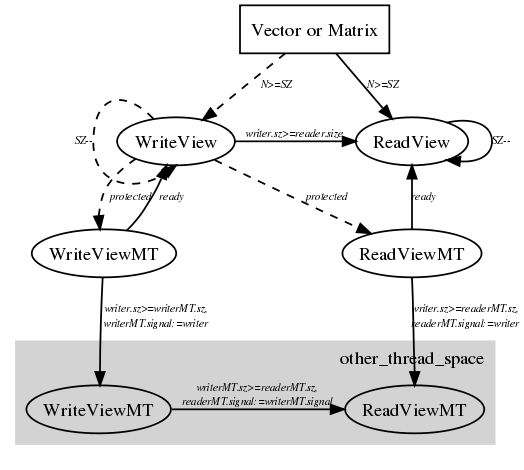
\includegraphics[width=3.3in]{view_concept}
\caption{View classes in libvina}
\label{fig:view}
\end{figure}
%%
\section{Runtime supports}
Basically, our static transformation does not incur any runtime
overhead. However, we need thread and synchronization to execute in
multi-threaded environment.

We implemented \emph{mt::thread} based on underlying pthread. A
simple C++ thread pool is developed to reduce cost of thread
creation. Because pthread does not have group-scheduling, we design
and implement a lightweight thread library (libSPMD) based on Linux
clone(2) and semaphore. Other advantages of libSPMD
is that it provides hook function to perform reduction and CPU binding. 
On GPU, we use OpenCL ~\cite{opencl} to obtain platform
independence. Many accelerators are scheduled or declared to
implement OpenCL, which might extend our approach to new
territories in the future.  Although the interfaces of threads
mentioned before are varying, our library can deal with them well.

In libvina, we implement barrier for both CPU and GPU. CPU's
implementation uses pthread conditional variables, while GPU counterpart
uses openCL's API function. GPU's barrier synchronizes
\emph{work-groups}. We still can not find a good method to generate kernel
barrier statement worked on \emph{work-items}.

We define a signal class to synchronize, which mimic
signal primitive on CellBE ~\cite{cellnetwork}. It is implemented by
conditional variable on x86. On GPU, we use \emph{event} of OpenCL to
achieve the same semantics.

\section{Source Transformations by Template}
We demonstrate transformation for two kinds of parallel pattern using
our template library. It is noting that we only apply recursion of
template classes on CPU. GPUs has dedicated hardware to map massive
number of threads on physical cores. In addition, we leverage OpenCL API on GPU, which
supports data parallelism and task parallelism. So transformation for
both SPMD and streaming becames on GPU are straightforward.

\subsection{SPMD}
Multithreading is dominant approach to utilize cloned computational resources. SPMD model is the most intuitive thread model.  SPMD is also
the foundation of streaming computation. There are numerous kernel functions in
multimedia applications and scientific computation which can 
exploit data parallelism by dividing task into smaller and independent
subtasks. This characteristic can be naturally expressed by libvina's
TF class. We implement \emph{mappar} and \emph{mapreduce} language constructs in Sequoia as template classes.

Fig.~\ref{lst:mappar} is a definition of \emph{TF\_mappar} for
x86. Template parameter \emph{Instance} is an adapter, which will be
described in next section. The last template
parameter of \textit{TF\_mappar} is a \emph{sentinel}. It determines control flow when
instantiation occurs. The second class in the figure is a template partial
specialization for the prime template, which generates concrete thread
to perform computation. It is noteworthy that the last two arguments
are true, which means that this class is multi-threaded and
leaf node version. \textit{aux::subview} is a meta-function to cut off
views. It could return a subset of the view or trivially return itself
according to the template parameters. Fig. ~\ref{lst:mappar}
gives a definition of arg0\_isomoph.

\begin{figure}[!htp]
\begin{minipage}[tb]{\linewidth}
\makebox[\textwidth]{\hrulefill}
\begin{small}
\begin{verbatim}
/*A TF class for mappar. no dependence exists
 *in subtasks of Instance. 
 */
template <class Instance,         /*problem*/
          int _K,      /*number of children*/
          bool _IsMT,     /*multi-threaded?*/
          bool __SENTINEL__ = Instance::_pred
>
struct TF_mappar {
 /*define recursively, evalue __SENTINEL__ 
  *using subtask's predicate
  */
 typedef TF_mappar<typename Instance::SubTask, 
       _K, _IsMT, 
       Instance::SubTask::_pred> _Tail;

 //determine whether Arg0 is isomorphic
 typedef typename mpl::or_<mpl::bool_
   <std::tr1::is_arithmetic
     <typename Instance::Arg0>::value>
   ,boost::mpl::bool_<
   std::tr1::is_same<typename Instance::Arg0, 
            typename Instance::SubTask::Arg0>
      ::value>
   >::type
 arg0_isomorph;

 //omitted ...

 static void 
 doit(const typename Instance::Arg0& arg0, 
      const typename Instance::Arg1& arg1, 
      typename Instance::Result& result)
 {
   for (int k=0; k < _K; ++k) {
    auto subArg0 = aux::subview<decltype(arg0), 
        arg0_dim::value, arg0_isomorph::value>
            ::sub_reader(arg0, k); 
    auto subArg1 = ... 
    auto subResult = ...
    
    //execute recursively
    _Tail::doit(*subArg0,*subArg1,*subResult);
   }
 }
};
/*A partial template specialization of
 *TF_mappar.
 */
template <class Instance, int  _K>
struct TF_mappar <Instance, _K 
             ,true          /*multithreaded*/ 
             ,true/*predicate is statisfied*/> 
{
 //omitted...
 static void 
 doit(const typename Instance::Arg0& arg0, 
   const typename Instance::Arg1& arg1,
   typename Instance::Result& result)
 {
   auto compF = Instance::computationMT();

   /*bind function object to a thread 
    *and run it.*/
   mt::thread_t leaf(compF, arg0, arg1, 
     aux::ref(result, result_arithm()));
 }
};
\end{verbatim}
\end{small}
\vspace{-3ex}\makebox[\textwidth]{\hrulefill}
\end{minipage}
\caption{TF class of \textsl{TF\_mappar}}\label{lst:mappar}
\end{figure}

\begin{figure}
\centering
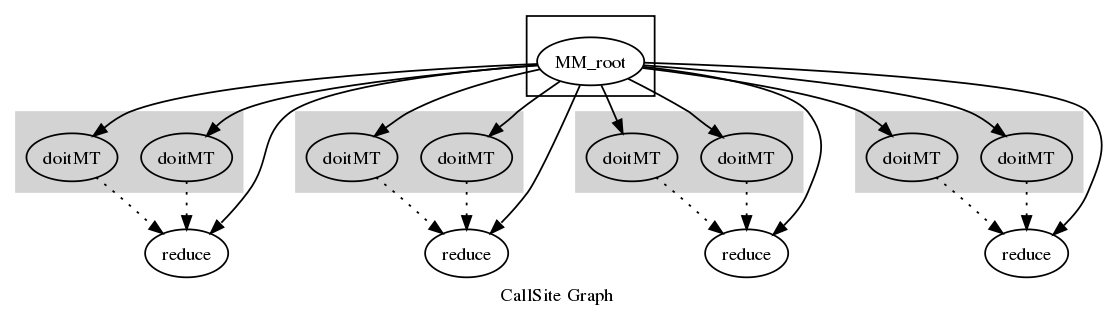
\includegraphics[width=3.3in]{test_matrix}
\caption{MM internal call graph}\label{fig:mm}
\end{figure}

Using the same mechanism, we define \emph{TF\_mapreduce}
class. Instance provides a reduction function, which will perform
after the barrier of loop. Fig.~\ref{fig:mm} is a cluster of
subprocedures generated by libvina after applying \emph{TF\_mapreduce} to a matrix multiplication
function. Subprocedure is the same concept of \emph{variant } in
\cite{sequoia, merge}. Template parameter \_K is 2 in this case because we intend
to perform this transformation for a dual core processor. \emph{mapreduce}
divides a matrix into 4 sub-matrices. The figure except dashed lines
is actually a call graph. Shadow box is multi-threaded environment and
subprocedures are executed simultaneously in pairwise. Dashed lines
indicate logical synchronization, implemented by a barrier.

\emph{mapseq} in Sequoia can be trivially implemented by
passing false to \emph{\_IsMT} parameter. Nested block is possible by
recursively defining \emph{TF classes}.

\subsection{Streaming and pipelining}
Streaming computation is a computer paradigm to perform massive parallel computation. It models data set as a \emph{stream}. Operations are usually organized in pipeline way to process in turn, while keeping stream in local storage. It can utilize multicore to perform computation in parallel and reduce external bandwidth.  Imagine~\cite{imagine} is typical architecture for
streaming computation.


More general streaming computation does not restrict to keep data
stationary. Pipeline processing inherently support heterogeneous
architectures or built-in ring network on chip ~\cite{cellbe, larrabee}. If specific processors
are exposed by platform and communication cost is manageable, developers
intend to leverage  them for performance or energy
advantages. Given the capability of metaprogramming, we have no problem to link external
computational devices as long as developers provide communication
layers. OpenCL is a programming model to support such kind of hybrid
execution for host CPU and its accelerators. 

Our template library provides two components to support streaming
computation. First, we provide  multi-threaded \emph{View}
classes depicted in Fig.~\ref{fig:view}. A \emph{ViewMT} class
contains a signal object to safeguard the ownership of underlying data
set. Second, libvina
defines a TF class listed in Fig.~\ref{lst:pipe} to perform
pipeline transformation. It synthesizes a group of function wrappers
and generates an execution chain with ViewMTs.  Fig. ~\ref{fig:viewmt}
depicts the scenario of pipelining in multi-threading environment. A
stage passes its ownership of data through ViewMT classes. Signal
classes take responsibility for waking up following stages.  It is noteworthy
that we intentionally leave the tail of recursion undefined. Our
template library has no idea how to deal with the output of pipeline. It is user's job
to define the last stage.

\begin{figure}[!htp]
\begin{minipage}[tb]{\linewidth}
\makebox[\textwidth]{\hrulefill}
\begin{small}
\begin{verbatim}
/*A TF class for pipeline. User need to define 
 *spacialization to handle the output of 
 *pipeline.
 */
template <typename... Stages>
struct TF_pipeline;

template <class P, typename... Tail>
struct TF_pipeline<P, Tail...> {
  typedef typename P::input_type in_t;
  typedef typename P::output_type out_t;
 
 static out_t doit(in_t in)
  {
    //static checker, omitted...
    TF_pipeline<Tail...>::doit( P::doit(in) );
  }
};  
\end{verbatim}
\end{small}
\vspace{-1ex}\makebox[\textwidth]{\hrulefill}
\end{minipage}
\caption{TF class of pipeline}\label{lst:pipe}
\end{figure}

\begin{figure}[htp]
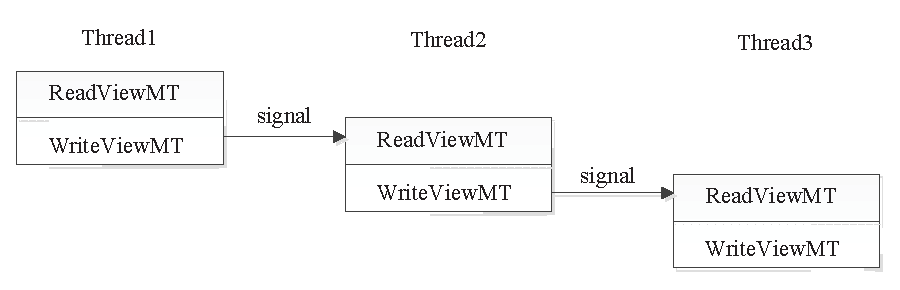
\includegraphics[width=3.1in]{viewmt}
\caption{ViewMT in pipelining}\label{fig:viewmt}
\end{figure}

%\subsection{Blocking}
\section{Adaption of TF classes}
TF classes manipulate instance classes. They transform the source code based on properties
of instances. \textit{e.g.} TF\_mapreduce utilizes the fact that
instance is divisible and reducible. TF\_pipeline utilizes the fact
that instances are combinable.  
User programmers are free to define their instance class to adapt libvina's TF class to their specific
problems. The only requirement is that they have to define the
properties using static members. Besides, TF classes need a couple of
interfaces to manipulate instance, including types and function
objects. We present two examples
of instance classes to demonstrate how to adapt customer's codes.

\begin{figure}[!htp]
\begin{minipage}[tb]{\linewidth}
\makebox[\textwidth]{\hrulefill}
\begin{small}
\begin{verbatim}
/*A adapter class for algorithm saxpy.
 */
template <class RESULT, class T,   class RHS, 
    template <typename, typename> class Func,
    template <typename, int>      class Pred,
               int K = 2 , bool IsMT = false>
struct ADAPTER_saxpy{
  //trait classes for type resolution
  typedef view_trait<RHS>    trait1;
  typedef view_trait<RESULT> trait_res;
  
  //types interfaces used by TF class
  typedef T                                Arg0;
  typedef typename trait1::reader_type     Arg1;
  typedef typename trait_res::writer_type 
                                         Result;
  //define TF class
  typedef TF_mappar<ADAPTER_saxpy/*instance*/
                    ,K, IsMT> Map;

  //define subTask
  typedef ReadView<T, trait1::READER_SIZE / K>
    SubRView1;
  typedef WriteView<T 
               ,trait_res::WRITER_SIZE / K>
    SubWView;
  typedef ADAPTER_saxpy<SubWView, T, SubRView1, 
                   Func, Pred, K, IsMT>
    SubTask;

  //pre-calculate predicate for TF class
  const static bool _pred = 
   Pred<T, trait1::READER_SIZE>::value;

  static void 
  saxpy(const T& alpha, const Arg1& lhs, 
       Result& rhs)
  {
    Map::doit(alpha, lhs, rhs);
  }
  
  static std::tr1::function
  <void (const T&, const Arg1&, Result&)>
  computation() 
  {
    return &(Func<Result, Arg1>::doit);
  }
};
\end{verbatim}
\end{small}
\vspace{-1ex}\makebox[\textwidth]{\hrulefill}
\end{minipage}
\caption{an adapter class for saxpy}\label{lst:adaptersaxpy}
\end{figure}
Fig.~\ref{lst:adaptersaxpy} is definition of an instance for
\emph{saxpy}. We will describe the algorithm later. The adapter defines TF\_mappar and call it in entry. 
The instance class recursively defines its subtask. Essentially, 
it defines how to divide the instance.
We evaluate the predicate \emph{Pred} in instance class and the value
is used by TF class as initializer of  template argument.
Type interfaces include Arg0, Arg1 and Result. A static function returns a function object which
instantiates function wrapper \emph{Func} using parameters in context. Fig.~\ref{lst:callsaxpy}
shows the usage of our adapter. Comparing with original call, new
entry keeps funciton name and arguments intact. However, inside of
TF\_MT::saxpy, a cluster of subprocedures are generated and executed
using threads..

\begin{figure}[!htp]
\begin{minipage}[tb]{\linewidth}
\makebox[\textwidth]{\hrulefill}
\begin{small}
\begin{verbatim}
//regular usage
vina::saxpy<VEC_TEST_TYPE, VEC_TEST_SIZE_N>
(7, x, result);
  
//use TF class to perform saxpy
typedef ADAPTER_saxpy<Writer, VEC_TEST_TYPE 
           ,TestVector         /*Vector type*/
           ,wrpSaxpy      /*function wrapper*/
           ,p_lt_cache_ll        /*predicate*/
           ,2/*K*/     ,true/*Multi-threaded*/
> TF_MT;
TF_MT::saxpy(7.0f, x, result);
\end{verbatim}
\end{small}
\vspace{-1ex}\makebox[\textwidth]{\hrulefill}
\end{minipage}
\caption{Call function with and without transformation}\label{lst:callsaxpy}
\end{figure}
Fig.~\ref{lst:callpipe} is an excerpt of program \textit{langpipe}. 
Fig.~\ref{lst:pipe} utilizes variadic template~\cite{vartemp} to
define recursion, which is one of C++0x features. The distinct of the
TF\_pipeline class in Fig.~\ref{lst:callpipe} is zero template
argument. We define a full template specialization for the last stage
of pipelining. The assignment of \textit{reader} is tricky. The type of
result is an regular view, while the type of argument \textit{in} is
uncertain. If it is a regular view, the assignment is trivial. If it is
a ViewMT class, the operation is blocking as depicted in Fig.~\ref{fig:viewmt}. \textit{MYPIPE} is the
synthesized class generated by TF\_pipeline. Each
\textit{translate} is independent instance, which complies with the
type interfaces defined in TF\_pipeline. Because instances access
contend data through ViewMT classes, it is combinable.

\begin{figure}[!htp]
\begin{minipage}[tb]{\linewidth}
\makebox[\textwidth]{\hrulefill}
\begin{small}
\begin{verbatim}
/*template full specialization for langpipe
 */
template<>
struct TF_pipeline<>
{
 static const bool _IsTail = true;
 typedef view_trait<STRING>::reader_type 
   READER;
  
 template <class U>
 static void output(U* in)
 {
   int i;
   /*U may be a ReadViewMT, in which case
    *the assignment is blocking operation.
    */
   READER reader = *(in);
   char output[READER::VIEW_SIZE+1];

   for(i=0; i<READER::VIEW_SIZE; ++i)
     out[i] = reader[i];
   out[i] = '\0';
   std::cout << out << std::endl;
 }
  
 template <class T>
 static void doit(T * in)
 {
   std::tr1::function<void (T*)> 
     func(&(output<T>));

   mt::thread_t thr(func, in);
 } 
};

//customize pipeline TF class
typedef TF_pipeline<
   translate<Eng2Frn 
            ,true/*Multi-threaded?*/
           >,
   translate<Frn2Spn, true>, 
   translate<Spn2Itn, true>,
   translate<Itn2Chn, true>
> MYPIPE;

//function call
MYPIPE::doit(&input);


\end{verbatim}
\end{small}
\vspace{-1ex}\makebox[\textwidth]{\hrulefill}
\end{minipage}
\caption{Call function before and after transformation}\label{lst:callpipe}
\end{figure}

%With the astonishing pace of core proliferation and architecture
%refinement, GPU has evolved to a pioneer of parallel computation,
%therefore, exploit of GPU bacomes urgent.

%OpenCL \cite{b12} is an industrial standard for heterogeous
%computation platforms.

%The prime downside of OpenCL is the obvious bias toward streaming
%architectures, which washes out many optimization techniques for
%traditonal architectures. Because our template
%approach is "meta'' programming techniqute,  it can mix OpenCL with
%other specialization methods. 

%Addionally, recursion is not supported by OpenCL in order to meet
%GPU's limitation.

\section{Experiments and evalution}
\subsection{Methodology}\label{sectn:method}
%compiler and libs
We implement our library in standard
C++\cite{c++03, c++0x}. Theoretically, any standard-compliance C++ compiler
should process our classes without trouble. New C++ standard (a.k.a C++0x)\cite{c++0x} adds a
lot of language features to ease template metaprogramming. Compilers
without C++0x supports need some workarounds to pass compilation
though, they do not hurt expressiveness. Consider the trend of C++,
development of template library like libvina should become easier
and smoother in the future.  Currently, C++0x has been partially supported by some mainstreaming
compilers.  We developed the library and tested using GCC 4.4.0.  The
first implementation of OpenCL was shipped by Mac OSX 10.6. The GPU performance is collected on that platform.

A couple of algorithms are evaluated for our template approach.  They
are typical in image processing and scientific fields. In
addition, we implemented a psuedo language translation program to
illustrate pipeline processing. The programs in experiments are listed
as follows:

\begin{itemize}
\item[\textit{saxpy}] Procedure in BLAS level 1. A scalar multiplies to a single precision vector, which contains 32 million elements.
\item[\textit{sgemm}] Procedure in BLAS level 3. Two 4096*4096 dense matrices multiply.
\item[\textit{dotprod}] Two vectors perform dot production. Each vector
  comprises 32 million elements.
\item[\textit{conv2d}] 2-Dimensional convolution operation on image.  The Image
  is 4094*4096 black-white format. Pixel is normalized as a single
  float ranging from 0.0 to 1.0.
\item[\textit{langpipe}] Pseudo-Multi-language translation. A word is translated from one language A to language B, and then another function will translate it from language B to language C, etc.
\end{itemize}

Two multicore platforms are used to conduct experiments. The hardware
platforms are summed up in Table.~\ref{tbl:mach}

\begin{table}[hbt]
\caption{Experimental platforms}\label{tbl:mach}
\begin{center}
\begin{tabular}{|l|l|l|l|l|r|}
\hline
\textbf{name}&\textbf{type}&\textbf{processors}&\textbf{memory}&\textbf{OS}\\
\hline
harpertown&SMP &x86 quad-core  &4G&Linux Fedora\\
                  &  server &   
2-way  2.0Ghz & &kernel 2.6.30\\
\hline
macbookpro&laptop &x86 dual-core &2G&Mac OSX\\
                    &           & 2.63Ghz         &  &Snowleopard\\
                   &           &GPU 9400m    &256M & \\
                    &           & 1.1Ghz   & &\\
\hline
\end{tabular} 
\end{center}
\end{table}
On harpertown, we link Intel Math kernels to perform BLAS procedures
except for conv2d. On macbookpro, we implemented all the algorithms on
our own. For CPU platform, we link libSPMD thread library to
perform computation. The library binds CPUs for each SPMD
thread and switch to realtime scheduler on Linux.  This configuration
helps eliminate the impact of OS scheduler and other processes in the system.
\subsection{Evaluation}
\subsubsection{Speedup of SPMD transformation on CPU}
\begin{figure}
\includegraphics{speedupx86.0}
\caption{Speedup on Harpertown}\label{fig:spdx86}
\end{figure}

Fig.~\ref{fig:spdx86} shows the speedup on harpertown. The blade
server contains two quad-core Xeon
processors. We experiment SPMD transformation for algorithms. \textit{saxpy} and
\textit{conv2d} apply  \emph{TF\_mappar} while \textit{dotprod} and \textit{sgemm} apply \emph{TF\_mapreduce}.

We obverse good performance scalability for programs
\textit{conv2d} and \textit{sgemm}. \textit{conv2d} does not have any dependences
and it can obtain about 7.3 times speedup in our experiments. sgemm
needs an extra reduction for each division operation. The final
speedup is about 6.3 times when all the cores are available. It is worth noting that we
observe almost two-fold speedup from sequence to dual core. However,
the speedup degrates to 3.3 time when execution
environment change to 4-core. Harpertown consists of  2-way quad-core processors,  Linux
can not guarantee that 4 subprocedures are executed within a physical
processor. Therefore, the cost of memory accesses and synchronization
increases from 2-core to 4-core platform. 

\textit{dotprod} and \textit{saxpy} reveal low speedup because non-computation-intensive
programs are subject to memory bandwidth.  In average, \textit{saxpy} needs one load and one 
store for every two operations. \textit{dotprod} has similar
situation. They quickly saturate memory bandwidth for SMP system and
therefore perform badly. Even though we fully parallelize those
algorithms by our template library. 
\subsubsection{Speedup of SPMD transformation on GPU}
\begin{figure}
\includegraphics{speedupgpu.0}
\caption{Speedup Comparing GPU with CPU}\label{fig:spdgpu}
\end{figure}

Fig.~\ref{fig:spdgpu} shows SPMD transformation results for GPU on
macbookpro. Programs run on host CPU  in sequence as
baseline. Embedded GPU on motherboard contains 2
SMs\footnote{Streaming Multiprocessor, each SM consists of 8 scalar processors(SP)}.
Porting from CPU to GPU, developer only need a couple of lines to change
templates while keeping algorithms same \footnote{
Because GPU code needs special qualifiers, we did modify kernel
functions a little manually.  Algorithms are kept except for sgemm. It is not easy
 to work out sgemm for a laptop, so we added blocking and SIMD
 instruments for CPU.}. As figure depicted,  computation-intensive programs
\textit{sgemm} and \textit{conv2d} still maintain their speedups. 4.5 to 5 times
performance boost is achieved for them by migrating to GPU.
In addition, we observe about 2 times performance boost for
\textit{saxpy}. Nvidia GPUs execute
threads in group of warp (32 threads) on hardware and it is
possible to coalesce memory accesses if warps satisfy
specific access patterns. Memory coalescence mitigates bandwidth issue
occurred on CPU counterpart. Because our program of \textit{dotprod} has fixed
step to access memory which does not fit any patterns, we can not
obtain hardware optimization without tweaking the algorithm.

\subsubsection{Comparison between different multicores}
\begin{table}[hbt]
\caption{Comparison of sgemm on CPU and GPU}\label{tbl:sgemm}
\begin{tabular}{|l|r|r|r|}
\hline
& baseline& CPU & GPU\\
\hline
\textbf{cores} &1 x86(penryn)& 8 x86(harpertown)& 2 SMs\\
\hline
\textbf{Gflops}& 2.64 &95.6&  12.0\\
\hline
\textbf{effectiveness}&12.6\%& 74.9\%&68.2\%\\
\hline
\textbf{lines of function}&63&unknown&21\\
\hline
\end{tabular}
\end{table}

Table.~\ref{tbl:sgemm} details \textit{sgemm} execution on CPU and GPU. Dense matrix
multiplication is one of  typical programs which have
intensive computation. Problems with this characteristic are the most
attractive candidates to apply our template-based approach.
Our template library transforms the \textit{sgemm} for both CPU and 
GPU. We choose sequential execution on macbookpro's CPU as
baseline. After mapping the algorithm to GPU, we directly obtains over
4.5 times speedup comparing with host CPU. Theoretically,  Intel Core
2 processor can issue 2 SSE instructions per cycle,  therefore, the
peak float performance is 21 Gflops on host CPU. We obtain 2.64 Gflops which
effectiveness is only 12.6\% even we employ quite complicated
implementation. On the other side, 12 Gflops is observed on GPU whose
maximal performance is roughly 17.6 Gflops.\footnote{$17.6Gflops = 1.1Ghz * 2(SM) *
  8(SP)$. nVidia declared their GPUs can perform a mad(multiply-add
  op) per cycle  for users who concern performance over precision. However, we can
  not observe mad hints bring any performance improvement in OpenCL. }
Although both column 2 and column 4 implement SIMD algorithm for
\textit{sgemm}, GPU's version is obviously easier and effective. It is
due to the dynamic SIMD and thread management from GPU
hardware~\cite{Fatahalian08} can significantly ease vector programming. Programmer can
implement algorithm in plain C and then replies on template
transformation for GPU.  Adapting \emph{TF\_mapreduce} template class
for GPU only need tens of lines code efforts. Like GPU template, we apply
\emph{TF\_mapreduce} to parallelize \textit{sgemm} procedure in MKL
for CPU. We observe 95.6 
Gflops and about 75\% effectiveness on harpertown server.

\subsubsection{Support streaming computation}
\begin{figure}[htp]
\includegraphics{pipeline.0}
\caption{Pipeline Processing for Psuedo Language Translation}\label{fig:pipe}
\end{figure}

Fig.~\ref{fig:pipe} demonstrates pipeline processing using our
template library. As described before, \textit{langpipe} simulates a
multilingual scenario. We apply template \emph{TF\_pipeline} listed in
Fig.~\ref{lst:pipe}. In our case, the program consists of  4 stages,
which can transitively translate English to Chinese\footnote{follow the 
  route: English  $\to$ French $\to$ Spanish $\to$ Italian $\to$
  Chinese}. Only the preceding stages complete,  it can proceed with
the next stages. The executing scenario is similar to Fig.~\ref{fig:viewmt}. We use bogus loop to consume $t \  \mu s$ on CPU. For each $t$, we iterate 500
times and then calculate the average consumptive time on harpertown. For
grained-granularity cases (20$\mu s$, 50$\mu s$, 100$\mu s$), we can obtain ideal
effectiveness in pipelining when 4 cores are exposed to the system.
\textit{i.e.} our program can roughly output one instance every $t\  \mu
s$. The speedup is easy to maintain when granularity is big. 100 $\mu s$ case ends up 54 $\mu s$ for each instance for 8 cores. 50  $\mu s$ case
bumps at 5 cores and then improves slowly along core increment. 20
$\mu s$ case also holds the trend of first two cases. 5 $\mu s$ case is
particular. We can not observe ideal pipelining until all 8
cores are available.  Our Linux kernel scheduler's granularity is 80
$\mu s$ in default. We think that the very fine granular tasks contend
CPU resources in out of the order. The runtime behavior presumably
incurs extra overhead. Many cores scenario helps alleviate the
situation and render regular pipeline processing.

\section{Related work}
As mentioned before, it is desirable to extend conventional programming languages to reflects new hardwares. Researches in the field have two major directions:
\begin{enumerate}
\item providing new library to support programming for concurrency
\item extending language constructs to extend parallel semantics
\end{enumerate}

First, library is a common method to extend language capability
without modifying grammar. Pthread library is a \textit{de facto} standard for
multi-threading on POSIX-compatible systems. The relationship between
pthread and native thread is straightforward. Therefore, abstraction
of pthread is far away from expressing parallelism and concurrency
naturally. Furthermore, the implementation of thread on hardware is
undefined in the standard, so it can not guarantee performance or even
correctness on some architectures \cite{Boehm05}. C++ community intend to develop parallel library while bearing
generic programming in mind. TBB~\cite{tbb} has a plenty of
containers and execution rules. Entities including partitioner and
scheduler in TBB are created at run time. In that case, key data
structures have to be thread-safe. Although TBB exploits task
parallelism or other sophisticated concurrency on general purpose
processors, the runtime overhead is relative high in data parallel
programs, especially in the scenario that many lightweight threads are
executing by hardware. Template-based approach we proposed is orthogonal to runtime parallel
libraries. We only explore parallelism which can be determined at
compile time, developers feel free to deploy other ways such as TBB to
farther improve programs.
 
%% MPI
%Another dominant parallel library is MPI in supercomputing community. It based on message-passing mechanism and SPMD model to execute parallel program. The difficulties of developing MPI programs are as notorious as pthread counterpart for programmers without sufficent training of parallel programming. 
%%

%OpenMP ~\cite{openmp} is designed for shared memory and has been shipped in almost every C/Fortran
%compilers.
%OpenMP can only perform Fork-Join parallel model.
%Source-to-Source transformation for optimization was reported by~\cite{Loveman77}, whose granularity of transformation  is
%statement.  Most of works have been merge in forms of IR in
%modern compilers. New source-to-source transformation compilers focus
%on function. 

The second choice for language community is to extend language constructs by
modifying compiler. They add directive or annotation to help compiler
transform source code. OpenMP compilers transform sequential code into
multi-threaded equivalence. The run-time is usually provides in the form of dynamic link library. Although it is simple and
portable, the performance is not optimal in most cases. Moreover, a
handful of directives in OpenMP leave small room for further improving
performance or scaling up to larger systems. Hybrid OpenMP with MPI is
possible though, difficulties surge. Sequoia supports
programming memory hierarchy. First of all, It targets execution
environment as a tree of machines, which an individual machine owns
its storage and computation unit. Second, it transforms a
\textit{task} into a
cluster of \emph{variants}. Target machine
is described in XML files. \cite{sequoia,
  sequoia-compiler} report  that Sequoia can transform programs
for CellBE, cluster while keeping competitive performance. That
is at expense of implementing one compiler for each platforms.
The primary drawback of Sequoia is that its language constructs can not cover common
parallel patterns such as pipeline or task queue. Besides, sequoia compiler
ignores type information to select optimal
implementation. Merge~\cite{merge} features a uniform runtime
environment for heterogeneous multicore 
systems in forms of task and variant. However, Merge only
support \emph{map-reduce} programming model. Its run-time overhead is not negligible for fine-granularity
parallelism. Methods mentioned before all need non-trivial efforts to
modify compilers. As discussed in \cite{sequoia}, the authors of the Sequoia were
still not clear whether the minimal set of primitives they provided provides can
sufficiently express dynamic applications. We doubt if it is worthwhile to
invest a compiler given the fact that template library can also
achieve the same functionalities.

%Libvina derived the idea of Sequoia to transform source code recursively. However, template metaprogramming utilizes existing mechanism in C++ compiler and is capable to express all the semantics in Sequoia programming language. Moreover, Sequoia can not leverage type system to specialize code. \textit{e.g.} Many modern processors usually provide SIMD instructions. Libvina could generate corresponding source based on predefined vector types. Sequoia compiler ignores this important information and simply relies on native compilers.
\section{Discussion and Future work}
The silicon industry has chosen multicore as new
direction. However, diverging multicore architectures enlarge the gap between algorithm-centric programmer and
computer system developers.  Conventional C/C++ programming language
can not reflect hardware essence any more.  Existing ad-hoc techniques
or platform-dependent programming language pose issues of generality
and portability. Source-to-source transformation can meet the challenge
and help tailor programs to specific multicore architectures.

%Not only the more processor cores but also
%elaborated memory hierarchy and exposed communication are adopted by
%new multicore architectures. More worse, 

We present a template metaprogramming approach to perform source-to-source
transformation for programs with rich information. Because it applies 
metaprogramming technique, template library is flexible enough to
apply any parallel
patterns and execution models. In addition, our approach
is extensible. Instead of modifying a compiler to add
annotations or language constructs, we implement the whole
functionalities by template mechanism. Template metaprogramming is
intimate for C++ programmers so they can extend the library to
facilitate proper parallel patterns and new architectural
features.  Our approach follows ISO C++ standards, which mean the
methodology is guaranteed to work across platforms.  Experiments shows
that our template approach can transform algorithms into SPMD threads
with competitive performance. These transformation are available for
both CPU and GPU, the cost of migration is manageable. We also
transform a group of standalone function wrappers into a
stream using our template library. It demonstrates that template
metaprogramming is powerful enough to support more than one parallel pattern.

%Our programming model bridges algorithm experts and diverging multcore
%architectures. Domain-specific experts focus on algorithms in form of
%conventional programming languages. They wrap functions to template
%classes and then pass them to \emph{TF class} as template parameter. Template
%mechniasm takes responisbility to transform source code according to
%their targets.

Streaming is an important computation model for innovative
multicore architectures. We partially exploit GPU functionality in this
paper though, transformation for GPU is quite
straightforward.  It is still unclear how many efforts need to
pay for a full-blown template library, which support
streaming computation. Libvina can only deal with regular
data. Future work on view class  will concentrate on supporting general operations like gather and scatter etc.  
Currently, kernel functions in GPU prohibit recursion. So we believe that
it is beneficial to introduce template recursion for GPU kernel functions. TF classes which support strip-mined memory access and loop iteration transformation are
particularly attractive for GPU targets because because  GPUs
provide memory coalescence for specific access patterns.

On CPU, source-to-source transformation should go on improving data
locality of programs. We plan to explore template approach to  generalize
blocking and tiling techniques.  It is also possible to re-structure
or prefetch data using template metaprograming accompanying with
runtime library.

General applications also contain a variety of static information to
optimize.The problem is that their memory footprints are irregular and
very hard to identify. It is desirable to explores new TF classes to facilitate
transforming source code close to target architectures using the static
information.

%GPU kernel function does not support recursion. It is not clear
%whether apply recursion to tranform kernel function can bring
%benefits.


% number - used to balance the columns on the last page
% adjust value as needed - may need to be readjusted if
% the document is modified later

\IEEEtriggeratref{11}

% The "triggered" command can be changed if desired:
%\IEEEtriggercmd{\enlargethispage{-5in}}

% references section

% can use a bibliography generated by BibTeX as a .bbl file
% BibTeX documentation can be easily obtained at:
% http://www.ctan.org/tex-archive/biblio/bibtex/contrib/doc/
% The IEEEtran BibTeX style support page is at:
% http://www.michaelshell.org/tex/ieeetran/bibtex/
%\bibliographystyle{IEEEtran}
% argument is your BibTeX string definitions and bibliography database(s)
%\bibliography{IEEEabrv,TCRef.bib}
%
% <OR> manually copy in the resultant .bbl file
% set second argument of \begin to the number of references
% (used to reserve space for the reference number labels box)

%\begin{thebibliography}{99}
%\setlength{\itemsep}{1mm}
%\bibitem{b1} Fatahalian, K., Knight, T., Houston, M., Erez, M., Horn, D.R., Leem, L., Park, J.Y., Ren, M., Aiken, A., Dally, W.J., Hanrahan, P.: Sequoia: Programming The Memory Hierarchy. SC2006
%\bibitem{b2} Knight, T. J., Park, J. Y., Ren, M., Houston, M., Erez, M., Fatahalian, K., Aiken, A., Dally, W. J., and Hanrahan, P. Compilation for Explicitly Managed Memory Hierarchies. PPoPP 2007
%\bibitem{b3} Aho, A., Sethi, R., Ullman, J.D., Lam, M.: Compilers: Principles, Techniques, and Tools. Addison-Wesley. 
%\bibitem{b4} Boehm, H.J.: Threads Cannot Be Implemented As a Library. PLDI '05
%\bibitem{b5} Drepper, U., Molnar, I.: The Native POSIX Thread Library for Linux. 2005
%\bibitem{b6} Veldhuizen, T. L.: C++ Template are Turing Complete. 
%\bibitem{b7} Saha, B., Zhou, X., Chen, H., Gao, Y., Yan, S., Rajagopalan, M., Fang, J., Zhang, P., Ronen, R., Mendelson, A.: Programming Model for Heterogeneous x86 Platform. PLDI '09.
%\bibitem{b8} C++ Standard Committee: ISO/IEC 14882:2003(E) Programming Languages — C++, 2003
%\bibitem{b9} Alexandrescu, A.: Modern C++ design: generic programming and design patterns applied, 2001
%\bibitem{b10} Abrahams, D., Gurtovoy, A.: C++ Template metaprogramming: Concepts, Tools, and Techniques from Boost and Beyond, 2004
%\bibitem{b11} Kapasi, U.J., Dally, W.J., Rixner, S., Owens, J.D., Khailany, B.: The Imagine Stream Processor. Proceeding of the 2002 International Conference on Computer Design.
%\bibitem{b12} Munshi, A., Khronos OpenCL Working Group, The OpenCL Specification ver.1.0.43, 2009
%\bibitem{b13} Goldberg, B.: Functional Programming Language, ACM Computing Surveys, 1996
%\bibitem{b14} Seiler, L., Carmean, D., Sprangle, E., Forsyth, T., Abrash, M., Dubey, P., Junkins, S., Lake, A., Sugerman, J., Cavin, R., Espasa, R., Grochowski, E., Juan, T., Hanrahan, P. 2008. Larrabee: A Many–Core x86 Architecture for Visual Computing. ACM Trans. Graph. August 2008
%\bibitem{b15} El-Ghazawi, T., Cantonnet, F., Yao, Y, Rajamony, R.: Developing an Optimized UPC Compiler for Future Architecture
%\bibitem{b16} Gurtovoy, A., Abrahams, D.: The BOOST C++ metaprogramming Library
%\bibitem{b17} C++ Standard Committee: ISO/IEC DTR 19768 Doc No. 2857, 2009
%\bibitem{b18} Stroustrup, B.: The C++ Programming Language (Spcial Edition) Addison Wesley. Reading Mass. USA. 2000. ISBN 0-201-70073-5
%\bibitem{b19} J. A. Kahle, M. N. Day, H. P. Hofstee, C. R. Johns, T. R. Maeurer, and D. Shippy: Introduction to the Cell Multiprocessor, IBM Journal of Research and Development 49, No. 4/5, 589-604, 2005
%\bibitem{b20} Official OpenMP Specifications, OpenMP Architecture
 % Review Board, 2002, http://www.openmp.org/specs/.
%\bibitem{b21}Linderman, M. D., Collins, J. D., Wang, H., Meng, T. H.:
 % Merge: A Programming Model for Heteogeneous Multi-core Systems. ASPLOS '08, March 1-5, Seattle, USA
%\bibitem{b22}Loveman, D., B: Program Improvement by Source-to-Source
%  Transformation, Journal  of the ACM, Vol.24, No. 1, Janulary
%  1977.pp 121-145
%\bibitem{b23}Nvidia: OpenCL Programming Guide for the CUDA
 % architecture, ver. 2.3

%\end{thebibliography}
% that's all folks
\bibliographystyle{ieeetran}
\bibliography{libvina}

\end{document}


